\documentclass[11pt,a4paper]{article}

\usepackage[margin=1in]{geometry}
\usepackage{mathptmx}
\usepackage{amsmath}
\usepackage{amssymb}
\usepackage{amsthm}
\usepackage{braket}
\usepackage{tikz}
\usepackage{quantikz}
\usepackage{enumitem}
\usepackage{hyperref}
\usepackage{xcolor}

\definecolor{circuitblue}{RGB}{40,80,160}

\hypersetup{
    colorlinks=true,
    linkcolor=circuitblue,
    urlcolor=circuitblue,
    citecolor=circuitblue
}

\theoremstyle{definition}
\newtheorem{definition}{Definition}[section]
\newtheorem{example}{Example}[section]
\newtheorem{theorem}{Theorem}[section]

\theoremstyle{remark}
\newtheorem*{intuition}{Intuition}
\newtheorem*{keypoint}{Key Point}

\pagestyle{plain}

\setlength{\parindent}{0pt}
\setlength{\parskip}{6pt}

\begin{document}

\begin{center}
    {\LARGE \textbf{Introduction to Quantum Hardware}}\\[8pt]
    {\large QML}\\[12pt]
    \hrule
\end{center}

\vspace{12pt}
\tableofcontents
\newpage

%% ========================================================
\section{Overview}
%% ========================================================

up until now weve been treating quantum computers as perfect mathematical objects --- u write a circuit, it runs exactly as specified, and u get the right answer. in reality, thats very far from the truth. real quantum hardware is noisy, limited in connectivity, has finite coherence times, and each gate introduces a small amount of error that accumulates as ur circuit gets deeper.

this lecture is about understanding the actual physical machines that run ur QML circuits. why does this matter? bcs the gap between ``ideal quantum computer'' and ``real quantum device'' determines whether ur fancy variational ansatz actually works or just produces garbage. if u design a 50-layer feature map but the hardware can only faithfully execute 10 layers before noise dominates, ur model is useless.

well cover the major hardware platforms --- superconducting qubits (IBM, Google), trapped ions (IonQ, Quantinuum), photonic systems (Xanadu), and neutral atoms (QuEra) --- with a deep dive into superconducting systems since thats wt most of u will use through IBM Quantum. well talk about gate fidelities, coherence times, qubit connectivity, and how all of this constrains the QML circuits u can actually run.

the key takeaway: hardware awareness isnt optional for QML. its the difference between circuits that work and circuits that dont.

%% ========================================================
\section{The Quantum Hardware Landscape}
%% ========================================================

there r four major approaches to building quantum computers that r actively being pursued by companies and research labs. each has different strengths and weaknesses, and these differences directly affect wt kinds of QML algorithms u can run.

\subsection{Overview of Platforms}

\begin{center}
\renewcommand{\arraystretch}{1.4}
\begin{tabular}{|l|c|c|c|c|}
\hline
\textbf{Property} & \textbf{Superconducting} & \textbf{Trapped Ions} & \textbf{Photonic} & \textbf{Neutral Atoms} \\
\hline
qubit type & transmon & atomic ions & photon modes & neutral atoms \\
\hline
connectivity & nearest-neighbor & all-to-all & reconfigurable & reconfigurable \\
\hline
gate speed & $\sim$10--100 ns & $\sim$1--100 $\mu$s & $\sim$1 ns & $\sim$0.1--1 $\mu$s \\
\hline
T1/T2 & $\sim$100--300 $\mu$s & $\sim$1--100 s & N/A (photon loss) & $\sim$1--10 s \\
\hline
2Q gate fidelity & 99--99.9\% & 99.5--99.9\% & $\sim$95--99\% & 99--99.5\% \\
\hline
scale (2024) & 100--1000+ Q & 20--56 Q & 100+ modes & 48--256 Q \\
\hline
key players & IBM, Google & IonQ, Quantinuum & Xanadu, PsiQuantum & QuEra, Pasqal \\
\hline
QML suitability & high (access) & high (connectivity) & niche (CV) & emerging \\
\hline
\end{tabular}
\end{center}

\begin{keypoint}
for QML, the two most important hardware properties r: (1) gate fidelity --- determines how deep ur circuits can be before noise dominates, and (2) connectivity --- determines how many SWAP gates u need to implement ur desired circuit, which adds depth and noise.
\end{keypoint}

%% ========================================================
\section{Superconducting Qubits --- Deep Dive}
%% ========================================================

superconducting qubits r the most widely deployed platform and the one most of u will interact with through IBM Quantum. lets understand how they actually work.

\subsection{The Josephson Junction}

the heart of a superconducting qubit is the josephson junction --- two superconducting electrodes separated by a thin insulating barrier (typically aluminum oxide, $\sim$1--2 nm thick).

\begin{definition}[Josephson Junction]
a josephson junction is a nonlinear, lossless circuit element with the current-phase relation:
\[
I = I_c \sin(\varphi)
\]
where $I_c$ is the critical current and $\varphi$ is the superconducting phase difference across the junction. the junction stores energy:
\[
U(\varphi) = -E_J \cos(\varphi)
\]
where $E_J = \frac{\bar{h} I_c}{2e}$ is the josephson energy (with $\bar{h}$ the reduced planck constant).
\end{definition}

why does this matter? bcs the nonlinearity of $\cos(\varphi)$ is wt gives us an anharmonic oscillator --- and thats wt lets us isolate two energy levels to use as a qubit.

\subsection{The Transmon Qubit}

a regular LC oscillator has equally spaced energy levels --- u cant address just two of them bcs a pulse that excites $\ket{0} \to \ket{1}$ would also excite $\ket{1} \to \ket{2}$. the transmon fixes this by replacing the linear inductor with a josephson junction.

the transmon hamiltonian is:
\[
\hat{H} = 4E_C(\hat{n} - n_g)^2 - E_J \cos(\hat{\varphi})
\]
where $E_C = \frac{e^2}{2C_\Sigma}$ is the charging energy, $\hat{n}$ is the number of cooper pairs, $n_g$ is the offset charge, and $C_\Sigma$ is the total capacitance.

the key design parameter is the ratio $E_J / E_C$. for a transmon, we want $E_J / E_C \gg 1$ (typically 50--100). this makes the qubit insensitive to charge noise (which is great for coherence) at the cost of reduced anharmonicity.

\begin{definition}[Anharmonicity]
the anharmonicity of a transmon is:
\[
\alpha = E_{12} - E_{01} = (E_2 - E_1) - (E_1 - E_0) \approx -E_C
\]
for a typical transmon, $\alpha / 2\pi \approx -300$ MHz, while the qubit frequency is $\omega_{01}/2\pi \approx 5$ GHz. this means the $\ket{0} \to \ket{1}$ transition is $\sim$300 MHz away from the $\ket{1} \to \ket{2}$ transition --- enough to selectively address the qubit subspace.
\end{definition}

\begin{intuition}
think of a transmon as a pendulum. a harmonic oscillator is like a spring --- all oscillation periods r the same regardless of amplitude. a pendulum has the property that larger swings take longer. this ``anharmonicity'' is wt lets u distinguish between different energy levels and treat the bottom two as a qubit.
\end{intuition}

the energy levels of the transmon r approximately:
\[
E_m \approx -E_J + \sqrt{8E_J E_C}\left(m + \frac{1}{2}\right) - \frac{E_C}{12}(6m^2 + 6m + 3)
\]
so the qubit frequency is:
\[
\omega_{01} = \frac{E_1 - E_0}{\bar{h}} \approx \frac{1}{\bar{h}}\left(\sqrt{8E_J E_C} - E_C\right)
\]

\subsection{Coupling Mechanisms}

individual qubits r useless without the ability to make them interact. there r two main coupling strategies in superconducting systems.

\textbf{capacitive coupling:} the simplest approach --- just put a capacitor between two transmons. this gives a fixed coupling:
\[
\hat{H}_{\text{int}} = g(\hat{a}_1^\dagger \hat{a}_2 + \hat{a}_1 \hat{a}_2^\dagger)
\]
where $g$ is the coupling strength (typically $g/2\pi \approx 1$--$10$ MHz) and $\hat{a}_i$, $\hat{a}_i^\dagger$ r the annihilation/creation operators for qubit $i$. the problem with fixed coupling is that qubits always interact, leading to unwanted ZZ crosstalk.

\textbf{resonator-mediated coupling:} a more sophisticated approach where qubits couple through a shared microwave resonator (bus resonator). in the dispersive regime (where qubit-resonator detuning $\Delta$ is much larger than the coupling $g$), the effective qubit-qubit interaction is:
\[
g_{\text{eff}} = \frac{g_1 g_2}{\Delta}
\]
this is how IBM connects qubits in their heavy-hex lattice --- each pair of connected qubits shares a coupling resonator.

\textbf{tunable couplers:} modern designs (used in Google's Sycamore and IBM's newer processors) include a tunable coupler between qubits that can turn the effective coupling on and off:
\[
g_{\text{eff}}(\Phi) = g_{\text{direct}} + \frac{g_{1c} g_{2c}}{\Delta_c(\Phi)}
\]
where $\Phi$ is the external flux threading the coupler. by tuning $\Phi$, u can set $g_{\text{eff}} = 0$ (qubits isolated) or $g_{\text{eff}} \neq 0$ (qubits interacting). this dramatically reduces crosstalk errors.

%% ========================================================
\section{Qubit Connectivity and Topology}
%% ========================================================

the physical layout of qubits and which pairs can directly interact is called the connectivity or topology. this is arguably the most important hardware constraint for QML bcs it determines how many SWAP operations u need.

\subsection{IBM's Heavy-Hex Lattice}

IBM uses a heavy-hex topology for their eagle (127 qubit) and heron (133 qubit) processors. here is a schematic:

\begin{center}
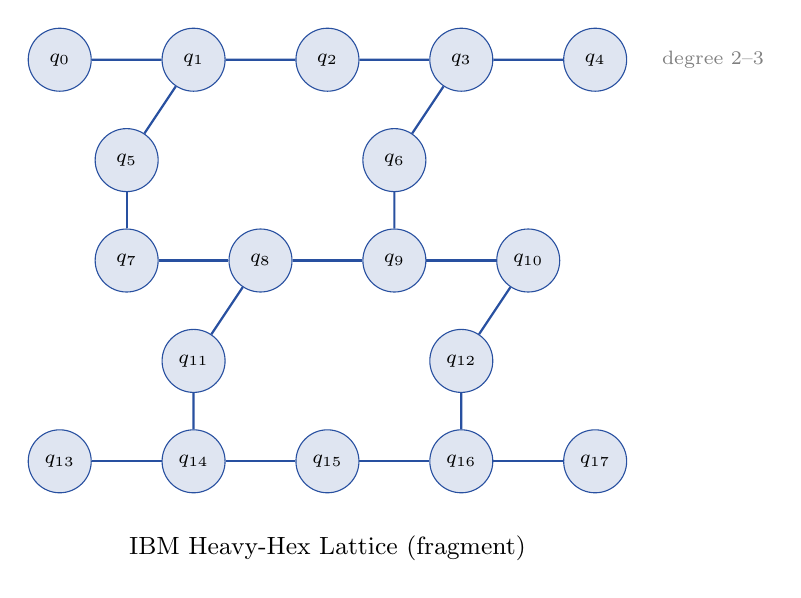
\begin{tikzpicture}[
    qubit/.style={circle, draw=circuitblue, fill=circuitblue!15, minimum size=8mm, inner sep=0pt, font=\scriptsize},
    conn/.style={draw=circuitblue, thick},
    scale=0.85
]
% top row
\node[qubit] (q0) at (0, 4) {$q_0$};
\node[qubit] (q1) at (2, 4) {$q_1$};
\node[qubit] (q2) at (4, 4) {$q_2$};
\node[qubit] (q3) at (6, 4) {$q_3$};
\node[qubit] (q4) at (8, 4) {$q_4$};

% bridge qubits (hanging down from top row)
\node[qubit] (q5) at (1, 2.5) {$q_5$};
\node[qubit] (q6) at (5, 2.5) {$q_6$};

% middle row
\node[qubit] (q7) at (1, 1) {$q_7$};
\node[qubit] (q8) at (3, 1) {$q_8$};
\node[qubit] (q9) at (5, 1) {$q_9$};
\node[qubit] (q10) at (7, 1) {$q_{10}$};

% bridge qubits (hanging down from middle)
\node[qubit] (q11) at (2, -0.5) {$q_{11}$};
\node[qubit] (q12) at (6, -0.5) {$q_{12}$};

% bottom row
\node[qubit] (q13) at (0, -2) {$q_{13}$};
\node[qubit] (q14) at (2, -2) {$q_{14}$};
\node[qubit] (q15) at (4, -2) {$q_{15}$};
\node[qubit] (q16) at (6, -2) {$q_{16}$};
\node[qubit] (q17) at (8, -2) {$q_{17}$};

% top row connections
\draw[conn] (q0) -- (q1);
\draw[conn] (q1) -- (q2);
\draw[conn] (q2) -- (q3);
\draw[conn] (q3) -- (q4);

% bridges from top to middle
\draw[conn] (q1) -- (q5);
\draw[conn] (q5) -- (q7);
\draw[conn] (q3) -- (q6);
\draw[conn] (q6) -- (q9);

% middle row connections
\draw[conn] (q7) -- (q8);
\draw[conn] (q8) -- (q9);
\draw[conn] (q9) -- (q10);

% bridges from middle to bottom
\draw[conn] (q8) -- (q11);
\draw[conn] (q11) -- (q14);
\draw[conn] (q10) -- (q12);
\draw[conn] (q12) -- (q16);

% bottom row connections
\draw[conn] (q13) -- (q14);
\draw[conn] (q14) -- (q15);
\draw[conn] (q15) -- (q16);
\draw[conn] (q16) -- (q17);

% labels
\node[below=4mm] at (4, -2.5) {\small IBM Heavy-Hex Lattice (fragment)};
\node[right=3mm, font=\scriptsize, text=gray] at (8.5, 4) {degree 2--3};
\end{tikzpicture}
\end{center}

\begin{keypoint}
in a heavy-hex lattice, every qubit has at most degree 3 (connects to at most 3 neighbors). this means u need a lot of SWAP gates to implement circuits that require interactions between distant qubits. for a QML circuit with all-to-all entanglement on $n$ qubits, u might need $O(n)$ SWAP gates per entangling layer.
\end{keypoint}

why heavy-hex? the low connectivity actually helps with reducing crosstalk errors. when qubits have fewer neighbors, theres less unwanted ZZ interaction, which makes it easier to achieve high gate fidelities. its a deliberate engineering tradeoff: worse connectivity but better per-gate quality.

\subsection{Google's Square Grid}

Google's Sycamore processor uses a 2D square grid where each qubit connects to 4 neighbors (except at edges). this gives better connectivity than heavy-hex but potentially more crosstalk.

the diameter of the graph (maximum shortest path between any two qubits) is smaller for a square grid, meaning fewer SWAPs r needed on average. for an $n \times n$ grid, the diameter is $2(n-1)$, while for heavy-hex its somewhat larger due to the sparse bridges.

\subsection{Impact on QML Circuits}

consider a simple QML ansatz that applies $\text{CNOT}$ between every pair of qubits in a 4-qubit system. on hardware with all-to-all connectivity (like trapped ions), this requires exactly 6 CNOT gates. on a linear chain, some of these CNOTs must be decomposed using SWAPs:

each SWAP gate costs 3 CNOT gates. so if ur ansatz needs $k$ non-native CNOT connections, and each requires on average $s$ SWAPs, ur actual two-qubit gate count is:
\[
N_{\text{2Q}} = N_{\text{native}} + 3 \cdot N_{\text{SWAP}} \cdot s
\]

\begin{example}
consider a 6-qubit QML circuit with circular entanglement ($q_0$-$q_1$-$q_2$-$q_3$-$q_4$-$q_5$-$q_0$) on a linear chain. 5 of the 6 CNOT gates r between neighbors and need no SWAPs. the $q_5$-$q_0$ gate requires routing through the entire chain, costing approximately 5 SWAP gates = 15 additional CNOT gates. so the total goes from 6 ideal CNOTs to $5 + 1 + 15 = 21$ actual CNOTs.
\end{example}

%% ========================================================
\section{Gate Fidelities}
%% ========================================================

gate fidelity measures how close the actual operation is to the ideal one. this is the single most important number for determining whether ur QML circuit will work.

\begin{definition}[Average Gate Fidelity]
for a quantum channel $\mathcal{E}$ that is supposed to implement a unitary $U$, the average gate fidelity is:
\[
F_{\text{avg}} = \int d\psi \, \bra{\psi} U^\dagger \mathcal{E}(\ket{\psi}\bra{\psi}) U \ket{\psi}
\]
where the integral is over uniformly distributed pure states.
\end{definition}

in practice, fidelities r measured using randomized benchmarking (RB), which gives the error per clifford gate, or more recently interleaved RB for specific gates.

\subsection{Typical Fidelity Numbers (2024)}

\begin{center}
\renewcommand{\arraystretch}{1.3}
\begin{tabular}{|l|c|c|}
\hline
\textbf{Gate Type} & \textbf{Typical Fidelity} & \textbf{Error Rate} \\
\hline
single-qubit gate (SX, RZ) & 99.9--99.99\% & $10^{-3}$--$10^{-4}$ \\
\hline
two-qubit gate (ECR, CX) & 99.0--99.9\% & $10^{-2}$--$10^{-3}$ \\
\hline
measurement (readout) & 98.0--99.5\% & $5 \times 10^{-3}$--$2 \times 10^{-2}$ \\
\hline
state preparation ($\ket{0}$) & 99.5--99.9\% & $10^{-3}$--$5 \times 10^{-3}$ \\
\hline
\end{tabular}
\end{center}

\subsection{How Fidelity Limits Circuit Depth}

heres the key calculation for QML. if each layer of ur circuit has $n_{1Q}$ single-qubit gates and $n_{2Q}$ two-qubit gates, and u have $L$ layers, the total circuit fidelity is approximately:
\[
F_{\text{circuit}} \approx F_{1Q}^{L \cdot n_{1Q}} \cdot F_{2Q}^{L \cdot n_{2Q}} \cdot F_{\text{meas}}^n
\]
where $n$ is the number of qubits measured.

taking logarithms and using $\ln(1-\epsilon) \approx -\epsilon$ for small error:
\[
\ln F_{\text{circuit}} \approx -L \cdot n_{1Q} \cdot \epsilon_{1Q} - L \cdot n_{2Q} \cdot \epsilon_{2Q} - n \cdot \epsilon_{\text{meas}}
\]

\begin{example}[Noise Budget for a QML Circuit]
say u have a 10-qubit QML circuit with $L$ layers, each layer having 10 single-qubit gates ($\epsilon_{1Q} = 10^{-3}$) and 9 two-qubit gates ($\epsilon_{2Q} = 5 \times 10^{-3}$). readout error is $\epsilon_{\text{meas}} = 10^{-2}$.

total error:
\[
\epsilon_{\text{total}} \approx L(10 \times 10^{-3} + 9 \times 5 \times 10^{-3}) + 10 \times 10^{-2}
\]
\[
= L(0.01 + 0.045) + 0.1 = 0.055L + 0.1
\]

for the circuit to have more signal than noise, we roughly need $\epsilon_{\text{total}} < 0.5$:
\[
0.055L + 0.1 < 0.5 \implies L < 7.3
\]

so u can run at most $\sim$7 layers. this is a hard constraint on ur QML ansatz depth.
\end{example}

\begin{center}
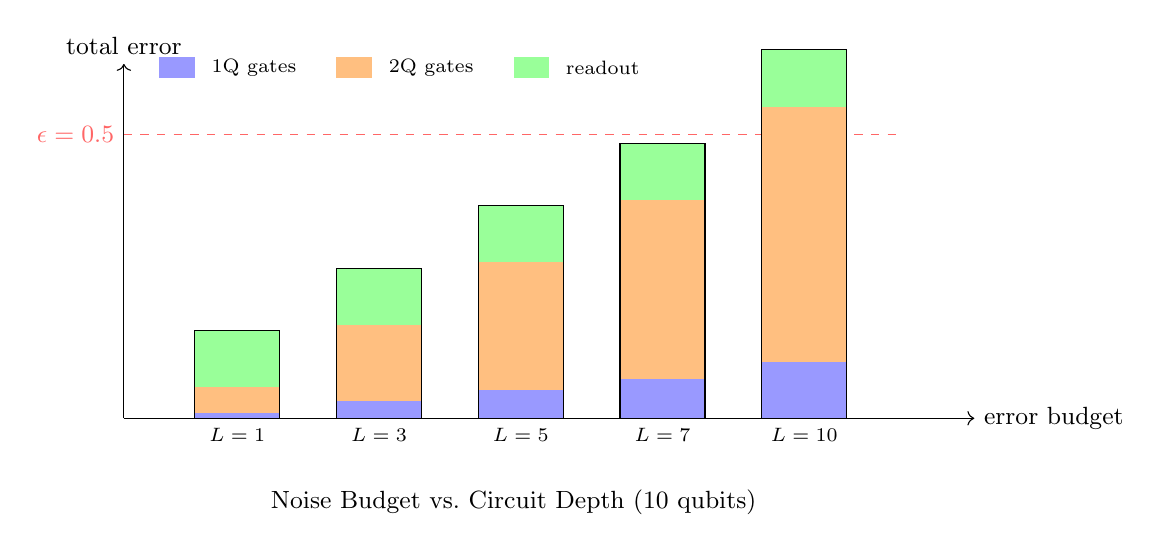
\begin{tikzpicture}[scale=0.9]
% noise budget bar chart
\draw[->] (0,0) -- (12, 0) node[right] {\small error budget};
\draw[->] (0,0) -- (0, 5) node[above] {\small total error};

% threshold line
\draw[dashed, red!60] (0, 4) -- (11, 4);
\node[left, red!60, font=\small] at (0, 4) {$\epsilon = 0.5$};

% bars for different layer counts
\foreach \l/\x in {1/1, 3/3, 5/5, 7/7, 10/9} {
    \pgfmathsetmacro{\oneerr}{0.01*\l}
    \pgfmathsetmacro{\twoerr}{0.045*\l}
    \pgfmathsetmacro{\measerr}{0.1}
    \pgfmathsetmacro{\total}{\oneerr + \twoerr + \measerr}
    \pgfmathsetmacro{\height}{\total * 8}
    \pgfmathsetmacro{\oneH}{\oneerr * 8}
    \pgfmathsetmacro{\twoH}{\twoerr * 8}
    \pgfmathsetmacro{\measH}{\measerr * 8}
    % 1Q errors
    \fill[blue!40] (\x, 0) rectangle (\x+1.2, \oneH);
    % 2Q errors (stacked)
    \fill[orange!50] (\x, \oneH) rectangle (\x+1.2, \oneH + \twoH);
    % measurement errors (stacked)
    \fill[green!40] (\x, \oneH + \twoH) rectangle (\x+1.2, \height);
    \draw (\x, 0) rectangle (\x+1.2, \height);
    \node[below, font=\scriptsize] at (\x+0.6, 0) {$L=\l$};
}

% legend
\fill[blue!40] (0.5, 4.8) rectangle (1, 5.1);
\node[right, font=\scriptsize] at (1.1, 4.95) {1Q gates};
\fill[orange!50] (3, 4.8) rectangle (3.5, 5.1);
\node[right, font=\scriptsize] at (3.6, 4.95) {2Q gates};
\fill[green!40] (5.5, 4.8) rectangle (6, 5.1);
\node[right, font=\scriptsize] at (6.1, 4.95) {readout};
\node[below=6mm, font=\small] at (5.5, -0.2) {Noise Budget vs.\ Circuit Depth (10 qubits)};
\end{tikzpicture}
\end{center}

%% ========================================================
\section{Coherence Times}
%% ========================================================

coherence times tell u how long a qubit can maintain quantum information before the environment destroys it. there r three key timescales.

\subsection{T1 --- Energy Relaxation}

\begin{definition}[$T_1$ Time]
$T_1$ is the timescale for energy relaxation --- the qubit spontaneously decays from $\ket{1}$ to $\ket{0}$. if u prepare $\ket{1}$ and wait time $t$, the probability of still being in $\ket{1}$ is:
\[
P_1(t) = e^{-t/T_1}
\]
this is analogous to the $T_1$ relaxation in NMR. for current transmons, $T_1 \approx 100$--$300 \, \mu$s.
\end{definition}

$T_1$ is caused by coupling to the electromagnetic environment --- the qubit radiates energy into modes it shouldnt be coupled to. dielectric loss in the substrate and junction is a major source.

\subsection{T2 --- Dephasing}

\begin{definition}[$T_2$ and $T_2^*$ Times]
$T_2$ (measured with a spin echo or Hahn echo sequence) captures dephasing --- the loss of phase coherence between $\ket{0}$ and $\ket{1}$. if u prepare $\ket{+} = \frac{1}{\sqrt{2}}(\ket{0} + \ket{1})$ and wait, the off-diagonal elements of the density matrix decay as:
\[
\rho_{01}(t) = \rho_{01}(0) \, e^{-t/T_2}
\]
$T_2^*$ (measured with a Ramsey experiment, no echo) includes both intrinsic dephasing and low-frequency noise:
\[
\frac{1}{T_2^*} = \frac{1}{2T_1} + \frac{1}{T_\varphi}
\]
where $T_\varphi$ is the pure dephasing time. always $T_2^* \leq T_2 \leq 2T_1$.
\end{definition}

\begin{intuition}
think of $T_1$ as the qubit ``forgetting whether its 0 or 1'' and $T_2$ as the qubit ``forgetting the phase angle between 0 and 1''. for QML, $T_2$ is usually more important bcs most quantum algorithms rely heavily on coherent superpositions, and dephasing kills those superpositions.
\end{intuition}

\subsection{What This Means for Circuit Depth}

the maximum number of gate layers u can execute is bounded by:
\[
L_{\max} \approx \frac{T_2}{t_{\text{gate}}}
\]
where $t_{\text{gate}}$ is the duration of one layer. for a two-qubit gate taking $\sim$300 ns and $T_2 \approx 200 \, \mu$s:
\[
L_{\max} \approx \frac{200 \times 10^3 \text{ ns}}{300 \text{ ns}} \approx 667 \text{ layers}
\]

but wait --- this is a theoretical maximum assuming perfect gates. in practice, gate errors accumulate much faster than decoherence, so the actual limit is usually set by gate fidelity (as we calculated above), not coherence time. on current hardware, gate errors limit u to $\sim$5--20 useful layers, well below the coherence limit.

%% ========================================================
\section{Calibration and Tuneup}
%% ========================================================

gates on a quantum computer r not fixed hardware components like logic gates on a classical chip. they r carefully calibrated microwave pulses, and their fidelity drifts over time.

\subsection{How Gates Are Calibrated}

a single-qubit gate on a transmon is implemented by a microwave pulse at the qubit frequency $\omega_{01}$. to calibrate, say, an $X$ gate (which should flip $\ket{0}$ to $\ket{1}$), u need to find:

\begin{enumerate}[label=(\arabic*)]
    \item \textbf{qubit frequency} $\omega_{01}$: found using spectroscopy (sweep microwave frequency, look for absorption)
    \item \textbf{pulse amplitude}: found using Rabi oscillations (sweep amplitude, find the $\pi$-pulse)
    \item \textbf{DRAG parameter}: corrects for leakage to the $\ket{2}$ state (derivative removal by adiabatic gate)
    \item \textbf{readout parameters}: discriminator calibration for telling $\ket{0}$ from $\ket{1}$ in the IQ plane
\end{enumerate}

two-qubit gates r even more involved --- for an ECR (echoed cross-resonance) gate, u need to calibrate the cross-resonance drive amplitude, duration, and phase, plus single-qubit corrections.

\subsection{Why Fidelities Drift}

qubit parameters drift due to:
\begin{itemize}[leftmargin=*]
    \item \textbf{TLS defects}: two-level systems in the substrate that couple to the qubit and shift its frequency on timescales of minutes to hours
    \item \textbf{temperature fluctuations}: small changes in the cryostat temperature affect qubit frequencies
    \item \textbf{cosmic rays}: high-energy particles can temporarily heat the chip and degrade all qubits simultaneously (recently observed by Google)
    \item \textbf{quasiparticle poisoning}: broken cooper pairs that tunnel across the junction and shift the qubit frequency
\end{itemize}

IBM recalibrates their systems approximately daily, and publishes calibration data (gate errors, $T_1$, $T_2$, readout errors) for each backend.

\begin{keypoint}
for QML experiments, always check the latest calibration data before submitting jobs. a qubit that was great yesterday might be terrible today. use the \texttt{BackendProperties} API in Qiskit to query current error rates and choose the best qubits for ur circuit.
\end{keypoint}

%% ========================================================
\section{IBM Quantum Systems}
%% ========================================================

lets look at the specific processors u can access through IBM Quantum.

\subsection{Eagle Processor (127 Qubits)}

the IBM Eagle processor, introduced in 2021, was the first to break 100 qubits. key specs:
\begin{itemize}[leftmargin=*]
    \item 127 qubits in heavy-hex topology
    \item median CNOT error: $\sim 1$--$2\%$
    \item median $T_1$: $\sim 100$--$200 \, \mu$s
    \item used in the ibm\_brisbane, ibm\_osaka, etc.\ backends
\end{itemize}

\subsection{Heron Processor (133 Qubits)}

the IBM Heron processor (2023--2024) represents a significant upgrade:
\begin{itemize}[leftmargin=*]
    \item 133 qubits, still heavy-hex
    \item tunable couplers (big improvement over fixed coupling in Eagle)
    \item native ECR gate replaced with improved two-qubit gate
    \item median two-qubit gate error: $\sim 0.3$--$0.5\%$ (roughly 3--5x better than Eagle)
    \item used in the ibm\_fez, ibm\_marrakesh, etc.\ backends
\end{itemize}

\subsection{IBM Roadmap}

IBMs roadmap includes:
\begin{itemize}[leftmargin=*]
    \item \textbf{Flamingo} (2025): modular architecture linking multiple chips via quantum interconnects
    \item \textbf{Starling/Blue Jay}: 200+ qubit processors with further error reduction
    \item \textbf{100,000 qubit target} by 2033
\end{itemize}

for QML, the key milestone is when two-qubit gate errors drop below $\sim 0.1\%$ --- at that point, circuits with $\sim$50+ meaningful layers become feasible, opening up much deeper ansatze.

%% ========================================================
\section{Quantum Volume and CLOPS}
%% ========================================================

how do u compare quantum computers in a hardware-agnostic way? two key metrics.

\subsection{Quantum Volume}

\begin{definition}[Quantum Volume]
quantum volume (QV) is defined as:
\[
\text{QV} = 2^{n^*}
\]
where $n^*$ is the largest number of qubits $n$ for which the system can successfully execute a random ``model circuit'' of depth $n$ with heavy output probability $> 2/3$.

the model circuit consists of $n$ layers, each being a random permutation followed by random SU(4) gates on pairs.
\end{definition}

\begin{intuition}
quantum volume measures the effective ``square'' of computation the machine can do. its $2^n$ where $n$ is the largest width such that a depth-$n$ circuit (on $n$ qubits) still produces meaningful results. higher QV = can run deeper, wider circuits faithfully.
\end{intuition}

current records (approximate, 2024):
\begin{itemize}[leftmargin=*]
    \item IBM: QV $= 2^{15} = 32768$ (achieved on smaller subsets of large processors)
    \item Quantinuum: QV $= 2^{20} = 1048576$ (H2 processor, 56 qubits)
    \item IonQ: QV $= 2^{15}$
\end{itemize}

note that trapped ion systems tend to achieve higher QV despite fewer qubits, bcs their all-to-all connectivity and high gate fidelities mean they can run deeper circuits.

\subsection{CLOPS --- Circuit Layer Operations Per Second}

\begin{definition}[CLOPS]
CLOPS measures the throughput of a quantum system:
\[
\text{CLOPS} = \frac{M \cdot K \cdot S \cdot D}{T_{\text{wall}}}
\]
where $M$ is the number of templates, $K$ is the number of parameter updates, $S$ is the number of shots, $D$ is the number of QV layers, and $T_{\text{wall}}$ is the total wall clock time including all classical overhead.
\end{definition}

\begin{keypoint}
CLOPS is critical for QML bcs variational algorithms like VQE and VQC require many iterations of the optimize-execute loop. if each iteration takes 10 minutes of wall clock time (including queue wait, compilation, execution, result retrieval), and u need 1000 iterations to converge, thats 7 days of wall time. high CLOPS = faster iteration = practical QML.
\end{keypoint}

IBM has pushed CLOPS from $\sim$1,000 (2021) to $\sim$100,000+ (2024) through improvements in:
\begin{itemize}[leftmargin=*]
    \item Qiskit Runtime: executing the optimization loop on classical computers co-located with the quantum hardware
    \item dynamic circuits: mid-circuit measurement and classical feedforward
    \item parallelized transpilation and faster data transfer
\end{itemize}

%% ========================================================
\section{Accessing Hardware: Qiskit Runtime Primitives}
%% ========================================================

the modern way to run circuits on IBM hardware is through Qiskit Runtime primitives. there r two:

\subsection{Estimator}

the Estimator primitive computes expectation values:
\[
\langle O \rangle = \text{Tr}[\rho \, O]
\]
where $\rho$ is the state prepared by ur circuit and $O$ is an observable (usually a Pauli string or sum of Pauli strings).

for QML, u use Estimator when ur model output is a continuous value (like a regression target or classification score computed as $\langle Z_0 \rangle$).

\subsection{Sampler}

the Sampler primitive returns quasi-probability distributions --- the probabilities of each bitstring outcome:
\[
p(x) = |\braket{x|\psi}|^2 \quad \text{for each bitstring } x
\]

for QML, u use Sampler when u need the full output distribution, e.g., for quantum kernel estimation where u need $|\braket{\phi(x_i)|\phi(x_j)}|^2$.

\subsection{Error Mitigation}

both primitives support built-in error mitigation:
\begin{itemize}[leftmargin=*]
    \item \textbf{twirled readout error extinction (TREX)}: mitigates measurement errors by randomizing the classical bit flip and correcting statistically
    \item \textbf{zero noise extrapolation (ZNE)}: runs the circuit at multiple noise levels (by inserting identity pairs of gates) and extrapolates to the zero-noise limit
    \item \textbf{probabilistic error cancellation (PEC)}: the most accurate but most expensive method --- requires full noise characterization and exponential sampling overhead
\end{itemize}

\begin{example}
a typical QML workflow on IBM hardware:
\begin{enumerate}[label=\arabic*.]
    \item define ur parameterized circuit $U(\theta)$ in Qiskit
    \item choose an observable (e.g., $Z_0$ for binary classification)
    \item create an Estimator with resilience level 1 (TREX + ZNE)
    \item inside the optimization loop: update $\theta$, call Estimator to get $\langle Z_0 \rangle$, compute loss, update $\theta$ via classical optimizer
    \item the Estimator handles transpilation, error mitigation, and shot management automatically
\end{enumerate}
\end{example}

%% ========================================================
\section{Why Hardware Matters for QML}
%% ========================================================

lets put it all together and understand why all of this directly constrains ur QML models.

\subsection{Feature Map Depth Constraints}

recall that a quantum feature map encodes classical data $x$ into a quantum state:
\[
\ket{\phi(x)} = U_{\phi}(x) \ket{0}^{\otimes n}
\]

the expressiveness of the feature map depends on its depth --- deeper circuits can create more complex features. but hardware limits the usable depth. if ur feature map requires $D$ layers of entangling gates, and the hardware can faithfully execute at most $D_{\max}$ layers, u need $D \leq D_{\max}$.

for current IBM hardware with two-qubit gate error $\sim 0.5\%$:
\[
D_{\max} \approx \frac{\ln(2)}{n \cdot \epsilon_{2Q}} \approx \frac{0.7}{10 \times 0.005} = 14 \text{ layers}
\]

(this is very rough --- the actual limit depends on the specific circuit structure and error mitigation used.)

\subsection{Noise Budget Analysis}

\begin{center}
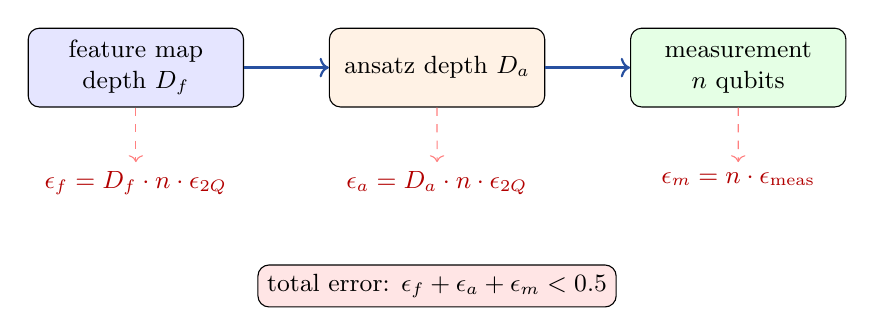
\begin{tikzpicture}[
    block/.style={draw, rounded corners, minimum width=2.5cm, minimum height=1cm, font=\small, text width=2.5cm, align=center},
    arrow/.style={->, thick, circuitblue},
    scale=0.85
]
% pipeline
\node[block, fill=blue!10] (feat) at (0, 0) {feature map depth $D_f$};
\node[block, fill=orange!10] (ansatz) at (4.5, 0) {ansatz depth $D_a$};
\node[block, fill=green!10] (meas) at (9, 0) {measurement $n$ qubits};

\draw[arrow] (feat) -- (ansatz);
\draw[arrow] (ansatz) -- (meas);

% error contributions
\node[below=1.2cm, font=\small, red!70!black] (e1) at (0, 0) {$\epsilon_f = D_f \cdot n \cdot \epsilon_{2Q}$};
\node[below=1.2cm, font=\small, red!70!black] (e2) at (4.5, 0) {$\epsilon_a = D_a \cdot n \cdot \epsilon_{2Q}$};
\node[below=1.2cm, font=\small, red!70!black] (e3) at (9, 0) {$\epsilon_m = n \cdot \epsilon_{\text{meas}}$};

\draw[->, dashed, red!50] (feat) -- (e1);
\draw[->, dashed, red!50] (ansatz) -- (e2);
\draw[->, dashed, red!50] (meas) -- (e3);

% total
\node[below=2.5cm, font=\small, draw, rounded corners, fill=red!10] at (4.5, 0) {total error: $\epsilon_f + \epsilon_a + \epsilon_m < 0.5$};
\end{tikzpicture}
\end{center}

the total error budget must be divided between:
\begin{enumerate}[label=(\arabic*)]
    \item \textbf{feature map}: needs enough depth to create useful features, but each layer costs noise
    \item \textbf{ansatz}: needs enough parameters for expressiveness, but each entangling layer costs noise
    \item \textbf{measurement}: fixed cost, scales with number of qubits
\end{enumerate}

this creates a fundamental tension in QML: u want deep circuits for expressiveness but shallow circuits for noise. next lecture well see how hardware-efficient ansatze try to get the most expressiveness per unit of noise.

\subsection{Circuit Depth Limits Per Platform}

\begin{center}
\renewcommand{\arraystretch}{1.3}
\begin{tabular}{|l|c|c|c|}
\hline
\textbf{Platform} & \textbf{2Q Error} & \textbf{Max Useful Layers (10Q)} & \textbf{QML Feasibility} \\
\hline
IBM Heron & $0.3\%$ & $\sim$20--25 & good for shallow ansatze \\
\hline
IBM Eagle & $1\%$ & $\sim$5--10 & marginal \\
\hline
Quantinuum H2 & $0.1\%$ & $\sim$50--70 & excellent \\
\hline
IonQ Forte & $0.3\%$ & $\sim$20--30 & good \\
\hline
\end{tabular}
\end{center}

%% ========================================================
\section{Trapped Ions}
%% ========================================================

trapped ion quantum computers use individual atomic ions (typically ytterbium-171 or barium-137) confined in electromagnetic traps. the qubit is encoded in two hyperfine energy levels of the ion.

\subsection{The Molmer--Sorensen (MS) Gate}

the native two-qubit gate for trapped ions is the Molmer--Sorensen (MS) gate:

\begin{definition}[MS Gate]
the MS gate implements:
\[
\text{MS}(\theta) = \exp\left(-i \frac{\theta}{4} \hat{\sigma}_x^{(1)} \otimes \hat{\sigma}_x^{(2)}\right)
\]
for $\theta = \pi/2$, this creates maximal entanglement:
\[
\text{MS}\left(\frac{\pi}{2}\right) \ket{00} = \frac{1}{\sqrt{2}}(\ket{00} - i\ket{11})
\]
\end{definition}

the MS gate works by using laser beams to couple the internal qubit states to the shared motional modes (phonons) of the ion chain. the key insight is that the phonon mode acts as a ``bus'' that mediates entanglement between any pair of ions, regardless of their physical distance in the chain.

\subsection{All-to-All Connectivity}

\begin{keypoint}
the biggest advantage of trapped ions for QML is all-to-all connectivity. any qubit can directly interact with any other qubit without SWAP routing. this means ur QML circuit runs exactly as designed --- no extra SWAP gates, no depth overhead, no additional noise from routing.
\end{keypoint}

for quantum kernel methods, this is particularly valuable. the kernel circuit:
\[
\ket{\psi} = U_\phi(x_2)^\dagger U_\phi(x_1) \ket{0}^{\otimes n}
\]
typically requires entangling gates between many qubit pairs. on trapped ions, the circuit depth for this is exactly the depth of the feature map. on superconducting qubits, it could be 2--3x deeper due to SWAP routing.

\subsection{Disadvantages}

\begin{itemize}[leftmargin=*]
    \item \textbf{slow gates}: MS gates take $\sim$100 $\mu$s vs.\ $\sim$50 ns for superconducting. this limits throughput.
    \item \textbf{scalability}: current systems have 20--56 qubits. scaling to 100+ requires shuttling ions between trap zones.
    \item \textbf{CLOPS}: much lower than superconducting systems, making iterative QML optimization slow.
\end{itemize}

%% ========================================================
\section{Photonic Quantum Computing}
%% ========================================================

photonic quantum computers use photons (particles of light) as qubits or, more commonly, as continuous-variable (CV) quantum systems.

\subsection{Continuous Variable Approach}

instead of discrete $\ket{0}$/$\ket{1}$ qubits, CV quantum computing uses the continuous quadratures of the electromagnetic field:
\[
\hat{x} = \frac{1}{\sqrt{2}}(\hat{a} + \hat{a}^\dagger), \qquad \hat{p} = \frac{i}{\sqrt{2}}(\hat{a}^\dagger - \hat{a})
\]

the native states r gaussian states (coherent states, squeezed states, thermal states) and the native operations r:
\begin{itemize}[leftmargin=*]
    \item \textbf{displacement}: $D(\alpha) = \exp(\alpha \hat{a}^\dagger - \alpha^* \hat{a})$
    \item \textbf{squeezing}: $S(r) = \exp\left(\frac{r}{2}(\hat{a}^2 - \hat{a}^{\dagger 2})\right)$
    \item \textbf{beam splitter}: $BS(\theta) = \exp\left(\theta(\hat{a}_1^\dagger \hat{a}_2 - \hat{a}_1 \hat{a}_2^\dagger)\right)$
    \item \textbf{Kerr interaction}: $K(\kappa) = \exp(i\kappa \hat{n}^2)$ (non-gaussian, needed for universality)
\end{itemize}

\subsection{Gaussian Boson Sampling}

xanadu's main demonstration has been gaussian boson sampling (GBS) --- sampling from the output distribution of a network of squeezed states interfering through a linear optical network:

\[
P(n_1, n_2, \ldots, n_M) = \frac{|\text{Haf}(A_S)|^2}{\prod_i n_i! \sqrt{\det(Q)}}
\]

where $\text{Haf}(A_S)$ is the hafnian of a submatrix determined by the output pattern. this is classically hard to simulate (under reasonable complexity assumptions).

\subsection{Photonic QML}

for QML, the CV approach offers a different kind of feature map. instead of encoding data into qubit rotations, u can encode it into displacements and squeezings:
\[
\ket{\phi(x)} = D(x_1) S(x_2) \cdots \ket{0}
\]

xanadu's PennyLane library supports CV quantum computing alongside qubit-based models.

%% ========================================================
\section{Neutral Atoms}
%% ========================================================

neutral atom quantum computers use arrays of individual atoms (typically rubidium or cesium) trapped in optical tweezers --- tightly focused laser beams that hold atoms in place.

\subsection{Rydberg Interaction}

the key mechanism for entanglement is the rydberg interaction. when an atom is excited to a rydberg state (very high principal quantum number $n \sim 50$--$100$), it has an enormous electric dipole moment, leading to strong van der waals interactions:

\[
V_{\text{vdW}}(r) = \frac{C_6}{r^6}
\]

where $C_6$ scales as $n^{11}$. this interaction creates a ``rydberg blockade'': if one atom in a pair is excited to the rydberg state, the other cannot be, bcs the interaction shifts it out of resonance.

\begin{definition}[Rydberg Blockade]
the blockade radius is:
\[
R_b = \left(\frac{C_6}{\bar{h} \Omega}\right)^{1/6}
\]
where $\Omega$ is the rabi frequency of the excitation laser. within $R_b$, at most one atom can be in the rydberg state. this naturally implements a controlled-Z type entangling gate.
\end{definition}

\subsection{Reconfigurable Arrays}

the killer feature of neutral atoms is reconfigurability. the optical tweezers can be rearranged in real time, allowing u to change the qubit connectivity between different parts of the circuit. this is huge for QML:
\begin{itemize}[leftmargin=*]
    \item run the feature map with one connectivity pattern
    \item rearrange atoms
    \item run the ansatz with a different connectivity pattern
    \item no SWAP gates needed, ever
\end{itemize}

QuEra's Aquila processor has demonstrated 256-atom arrays with reconfigurable geometry.

\subsection{Native Gates}

the native operations r:
\begin{itemize}[leftmargin=*]
    \item global rotations: all qubits rotate simultaneously ($R_x(\theta)$, $R_y(\theta)$)
    \item local addressing: individual qubit rotations (emerging capability)
    \item CZ-type gates via rydberg blockade: automatic for atoms within $R_b$
\end{itemize}

for QML, the global rotation constraint means u design ansatze differently --- instead of individual rotations per qubit, u use global pulses and rely on the interaction pattern for expressiveness. this is actually well-suited to QAOA-style circuits.

%% ========================================================
\section{Platform Comparison for QML}
%% ========================================================

lets compare all platforms specifically for QML workloads.

\begin{center}
\renewcommand{\arraystretch}{1.4}
\small
\begin{tabular}{|l|c|c|c|c|}
\hline
\textbf{QML Criterion} & \textbf{Supercond.} & \textbf{Trapped Ions} & \textbf{Photonic} & \textbf{Neutral Atoms} \\
\hline
kernel circuit depth & moderate & low (all-to-all) & N/A (CV) & low (reconfig.) \\
\hline
VQC iteration speed & fast (high CLOPS) & slow & moderate & moderate \\
\hline
max useful qubits & 50--127 & 20--56 & 100+ modes & 48--256 \\
\hline
SWAP overhead & high & none & N/A & minimal \\
\hline
error mitigation & mature (Qiskit) & developing & limited & developing \\
\hline
software ecosystem & excellent (Qiskit) & good (tket) & good (PennyLane) & emerging \\
\hline
cloud access & easy (IBM Q) & available (Azure) & available (Xanadu) & limited \\
\hline
best QML use case & VQC (iterative) & kernels & CV QML & QAOA, optimization \\
\hline
\end{tabular}
\end{center}

\begin{keypoint}
there is no single ``best'' quantum hardware for QML. the right choice depends on ur specific algorithm:
\begin{itemize}[leftmargin=*]
    \item iterative VQC training with many optimization steps $\to$ superconducting (high CLOPS)
    \item quantum kernel methods with all-to-all entanglement $\to$ trapped ions (no SWAP overhead)
    \item continuous-variable QML or GBS-based kernels $\to$ photonic
    \item QAOA-style optimization with geometry-dependent interactions $\to$ neutral atoms
\end{itemize}
\end{keypoint}

%% ========================================================
\section{Practical Considerations}
%% ========================================================

\subsection{Choosing Qubits on a Backend}

not all qubits on a processor r equally good. typical variation on a 127-qubit Eagle:
\begin{itemize}[leftmargin=*]
    \item best qubits: 2Q error $\sim 0.5\%$, $T_1 \sim 300 \, \mu$s
    \item worst qubits: 2Q error $\sim 3\%$, $T_1 \sim 30 \, \mu$s
    \item thats a 6x variation in quality across the same chip
\end{itemize}

Qiskit's transpiler can automatically map ur circuit to the best available qubits using the \texttt{optimization\_level=3} setting.

\subsection{Shot Budget}

each circuit execution (shot) gives one sample from the output distribution. to estimate an expectation value $\langle O \rangle$ to precision $\epsilon$, u need:
\[
N_{\text{shots}} = O\left(\frac{\text{Var}(O)}{\epsilon^2}\right)
\]

for a Pauli observable $O$ with eigenvalues $\pm 1$, the variance is at most 1, so:
\[
N_{\text{shots}} \geq \frac{1}{\epsilon^2}
\]

for $\epsilon = 0.01$ (1\% precision), u need $\sim$10,000 shots. at 1000 CLOPS, this takes about 10 seconds. reasonable for one circuit, but a VQC with 100 parameters might need 100 gradient evaluations per step $\times$ 200 steps = 20,000 circuit evaluations. thats $\sim$56 hours of continuous execution.

\subsection{Error Mitigation Overhead}

error mitigation helps but costs additional shots:
\begin{itemize}[leftmargin=*]
    \item \textbf{TREX}: minimal overhead ($\sim$2x shots)
    \item \textbf{ZNE}: moderate overhead ($\sim$3--5x shots, running at multiple noise levels)
    \item \textbf{PEC}: exponential overhead ($\sim e^{2\gamma}$ where $\gamma$ is the total noise strength)
\end{itemize}

for a practical QML experiment, TREX + ZNE is usually the sweet spot --- enough mitigation to get useful results without blowing up the shot budget.

%% ========================================================
\section{Summary and Outlook}
%% ========================================================

key takeaways from this lecture:

\begin{enumerate}[label=\arabic*.]
    \item quantum hardware is noisy and limited --- this is the dominant constraint on QML today
    \item superconducting qubits (IBM) r the most accessible platform with the best software ecosystem
    \item gate fidelity (especially 2Q gates) determines ur maximum circuit depth, which is typically 5--25 useful layers on current hardware
    \item qubit connectivity determines SWAP overhead --- heavy-hex topology means many extra gates for non-local interactions
    \item coherence times ($T_1$, $T_2$) set a theoretical upper bound on circuit depth, but in practice gate errors r the bottleneck
    \item quantum volume and CLOPS r the key metrics for comparing hardware for QML workloads
    \item different platforms have different strengths: superconducting for speed, trapped ions for connectivity, photonic for CV, neutral atoms for reconfigurability
    \item always check calibration data and choose qubits carefully when running on real hardware
\end{enumerate}

next lecture well tackle the natural follow-up question: given all these hardware constraints, how do we design ansatze that actually work? thats the topic of hardware-efficient ansatze for QML.

\end{document}
